\chapter{GDPR}

The \textbf{General Data Protection Regulation (GDPR)} is a
comprehensive data protection law that replaced the Data Protection
Act 1998. It came into effect on \textbf{May 25, 2018} and aims to
strengthen the protection of personal data for individuals within the
EU, without enforcing any compulsory measures for data protection.

GDPR is a \textbf{Regulation}, meaning it has direct applicability
across all EU member states. It consists of two main components:
\begin{itemize}
    \item \textbf{Articles}: These are the legally binding provisions
      that form the core of the regulation.
    \item \textbf{Recitals}: These are explanatory notes within the
      body of the GDPR that provide context and guidance for
      interpreting the Articles.
\end{itemize}

The \textbf{Article 29 Working Party} serves as the EU's central
guidance body for GDPR-related issues, offering advice and
clarifications on the implementation and interpretation of the
regulation.

Each country has a \textbf{Supervisory Authority} responsible for
monitoring the application of GDPR and protecting the rights of
individuals. Notable examples include:
\begin{itemize}
    \item \textbf{Italy}: \textit{Garante per la protezione dei dati
      personali} – \url{https://www.garanteprivacy.it/}
    \item \textbf{United Kingdom}: \textit{Information Commissioner's
      Office (ICO)} – \url{https://www.ico.org.uk/}
    \item \dots
\end{itemize}

\section{Applicability}

The \textbf{GDPR} applies to any organization that processes or
controls the personal data of \textbf{EU residents}, regardless of the
organization's \textbf{size} or \textbf{location} (as established in
\textbf{Article 3} of the regulation). This extraterritorial scope
means that even non-EU organizations \textbf{must comply} with GDPR if
they handle the personal data of individuals residing within the EU.

For comparison, the \textbf{California Consumer Privacy Act (CCPA)} —
later amended by the \textbf{California Privacy Rights Act (CPRA)} in
2023 — protects only \textbf{California residents}. The CCPA/CPRA
applies specifically to \textbf{for-profit businesses} that do
business in California and meet at least one of the following
criteria:
\begin{itemize}
    \item Have a \textbf{gross annual revenue} of over \textbf{\$25
      million}.
    \item \textbf{Buy, sell, or share} the personal information of
      \textbf{100,000 or more} California residents or households.
    \item Derive \textbf{50\% or more of their annual revenue} from
      selling the personal information of California residents.
\end{itemize}
As a reference, a non-profit organization or a small business could
sell the personal data of it's customers and still not be subject to 
the CCPA/CPRA.

\section{Personal data}
\begin{boxH}
  With personal data one refers to any information relating to an
  identified or identifiable living person.
\end{boxH}
Some notable example of personal data include:
\begin{itemize}
  \item Human Resources records
  \item CCTV images of a student
  \item photograph of myself
  \item e-mail with me cc’d
  \item confidential opinions written about me by my supervisor
  \item even anonymised monitoring data
\end{itemize}
The status of personal data could be valid for both automated (i.e.
computer-based, like logs for network monitors) and manual filing
systems.

\subsection{Sensitive personal data}
Sensitive Personal data, also known as Special Category Personal Data
(art. 9.1), is a subset of personal data that is subject to additional 
protection under the GDPR.

The data that is considered to be sensitive personal data includes:
\begin{itemize}
  \item racial / ethnic origin
  \item political opinions
  \item religious / philosophical beliefs
  \item trade union membership
  \item genetic or biometric data
  \item health
  \item sex life / sexual orientation
\end{itemize}
Criminal offences and convictions are not included in this list but
separated out and similar extra safeguards put in place at Art.10.

\section{Data controller/processor/processing}
The data controller says \textbf{how and why} personal data is
processed. The data processor acts on the controller’s behalf,
processing the data, which is any activity with personal data, 
including collecting, storing, using, deleting, sharing.

\subsection{Data Properties}

The \textbf{GDPR} defines specific properties that personal data must
adhere to during processing. These principles ensure that data is
handled in a way that respects the rights and privacy of individuals.

\paragraph{Lawful, Fair, and Transparent Processing}  
Data must be processed \textbf{lawfully, fairly, and transparently}.  
\begin{itemize}
    \item \textbf{Lawful:} Data processing must not breach other laws
      and must comply with \textbf{Articles 6 and 9} of GDPR, which
      define the legal bases for processing personal data. 
    \item \textbf{Fair and Transparent:} Data subjects must be made
      aware of how their data is being processed (e.g., through
      privacy notices) and must feel they are being treated fairly.
\end{itemize}

\paragraph{Purpose Limitation}  
Data must be \textbf{collected for specified, explicit, and legitimate
purposes} and cannot be further processed in ways that are
\textbf{incompatible} with those purposes. When requesting consent,
it must be specific to a clearly defined purpose and \textbf{cannot be
reused} for other unrelated purposes.

\paragraph{Data Minimisation}  
Data must be \textbf{adequate, relevant, and limited} to what is
necessary for the purposes for which it is processed. Organizations
should avoid collecting excessive data and only request the minimum
amount needed to achieve their purpose.  

\paragraph{Data Accuracy}  
Data must be \textbf{accurate and kept up to date} where necessary.
Organizations should design and implement procedures to update data to
avoid errors or outdated information.  

\paragraph{Storage Limitation}  
Data must be stored in a form that \textbf{permits identification of
the subject only for as long as necessary} to achieve the purpose of
processing. Organizations should periodically review and delete "old"
data to avoid indefinite storage.  

\subsection{Breach Reporting}

\begin{boxH}
  A \textbf{personal data breach} refers to any breach of security
  that results in the \textbf{destruction, alteration, unauthorized
  disclosure, or access} to personal data. GDPR establishes specific
  obligations for organizations in the event of such a breach.
\end{boxH}

If the breach is likely to pose a \textbf{risk to the rights and
freedoms of individuals}, the organization must notify the
\textbf{Supervisory Authority} within \textbf{72 hours} of becoming
aware of it. This requirement is detailed in \textbf{Article 33} of
the GDPR.

If the breach is likely to result in a \textbf{high risk to the rights
and freedoms of individuals}, affected individuals must also be
notified. This ensures that individuals can take appropriate action to
protect themselves from potential harm.  

Failure to comply with the breach reporting obligations can result in
significant penalties. Organizations may face \textbf{fines of up to
4\% of their annual worldwide turnover} from the previous financial
year, with a maximum fee of \textbf{EUR 20 million}, as specified in
\textbf{Article 83} of the GDPR.  

\section{Data transfers}
GDPR imposes restrictions on the transfer of personal data outside the
EEA, to third countries or international organisations.

The Commission may designate non-EEA countries as having adequate
level of data protection otherwise must ensure appropriate safeguards
with agreements (e.g. Standard Commercial Clauses, SCC) like the EU-US
Privacy shield, which allows US companies to self-certify that they 
meet the EU data protection requirements.

\subsection{Information Lifecycle Management}
From a cybersecurity point of view, we have to protect the information
lifecycle management, which includes the following steps:
\begin{enumerate}
  \item Information Asset Registers (IAR)
  \item Data Flow Mapping (DFM)
  \item Risk Assessment(s)
  \item Privacy Notice(s)
  \item System Level Security Policy (SLSP)
\end{enumerate}

\section{Article 25}
Article 25 of the GDPR outlines the requirements for data protection 
by design and by default.

\subsection{Article 25, paragraph 1}
Article 25, paragraph 1, requires organizations to \textbf{consider
the state of the art} when implementing data protection measures. This
means that even if a protection system was considered sufficient at a
given point in time, it must be periodically reviewed to ensure it
aligns with current technological advancements. Failure to maintain
compliance with the state of the art can result in the system being
deemed inadequately protected.

The article emphasizes a \textbf{risk-based approach} to data
protection. Organizations must first perform a \textbf{risk analysis}
to identify potential threats and vulnerabilities. Based on the
analysis, they must then implement protection measures that are
\textbf{proportionate to the identified risks}. This approach ensures
that resources are focused on mitigating the most critical threats.

Article 25 requires the implementation of \textbf{both technical and
organizational measures} to achieve effective data protection.
\textbf{Technical measures} may include encryption, access control,
and secure data storage.  \textbf{Organizational measures} focus on
training personnel, promoting privacy awareness, and monitoring
employee behavior to ensure compliance.  

The article highlights the need to \textbf{integrate data protection
measures} into the design and operation of processing activities,
rather than treating them as add-ons. This integration ensures a
holistic approach to data protection and aligns with the principle of
\textbf{data protection by design and by default}, as mandated by
GDPR.

\subsubsection{State of the art}
We know that millions of new attacks are created every month, and
patches require a lot of time to be actually implemented and thus
close the window of exposure. This calls for periodic reviews and
updates of the security measures in place.

\begin{figure}[H]
  \centering
  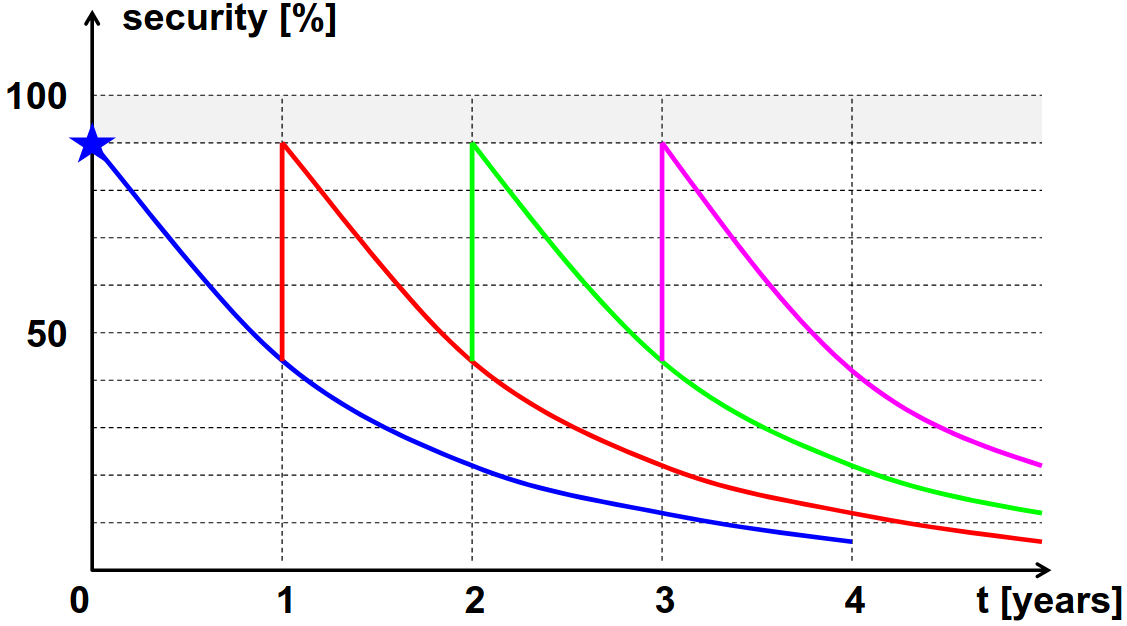
\includegraphics[width=0.8\textwidth]{img/periodic reviews.png}
  \caption{Periodic reviews}
  \label{fig:periodic reviews}
\end{figure}

Take a look at figure \ref{fig:periodic reviews} for a visual
representation of the periodic reviews. Imagine the system was created
at time 0 achieving a certain amount of security which cannot achieve
100\%. Given the number of new attacks, vulnerability, malware, etc.
The statistics tells that we are losing nearly half of the
effectiveness every year. In at most 4 years the security drops
towards 0. The review should be done periodically in a time frame less
than 1 year

\subsection{Article 25, paragraph 2}
Article 25, paragraph 2, requires that \textbf{data protection
mechanisms be activated by default}, not as optional settings.
Organizations must demonstrate that their technical solutions are
configured to ensure maximum privacy without requiring user
intervention. This principle directly supports the concept of
\textbf{data minimization}, ensuring that only personal data necessary
for a specific task is processed.  

This obligation applies to several aspects of data handling:  
\begin{itemize}
  \item \textbf{Amount}: The volume of data collected must be limited
    to what is essential for the task.  
  \item \textbf{Extent}: The type of processing applied to the data
    must be constrained to what is necessary.  
  \item \textbf{Time}: Data should only be stored for as long as
    required for its intended purpose.  
  \item \textbf{Accessibility}: Access to the data must be limited to
    only those who need it, adhering to the \textbf{principle of
    need-to-know}.  
\end{itemize}

A common issue in organizations is the use of \textbf{legacy
databases}, where access to all data is technically possible, but
restrictions are enforced only through query-level access control. For
instance, employees may be given pre-compiled queries to access
specific data, but if they modify these queries, they could
potentially access more data than intended. This approach is not
compliant with GDPR. To address this, organizations are encouraged to
\textbf{restructure their database design} by creating separate tables
for distinct functions or at least employing \textbf{database views}
that enforce strong access control measures.  

When dealing with social media, special attention is required since
social platforms are inherently public. GDPR mandates that, \textbf{by
default, personal data should not be accessible to an indefinite
number of people}. For example, when a user shares content on social
media, the platform must ensure that the content is not automatically
visible to everyone unless the user explicitly consents. This requires
an additional step of user intervention to grant permission for public
sharing.  

\subsection{Article 25, paragraph 3}
Article 25, paragraph 3, introduces the concept of
\textbf{certification mechanisms} to demonstrate GDPR compliance.
Organizations can voluntarily seek certification for their data
protection measures. This certification provides formal validation of
compliance, offering evidence of the organization’s \textbf{good faith
efforts} to protect personal data.  

However, the certification process has its limitations:  
\begin{itemize}
  \item \textbf{Voluntary, Not Mandatory}: Certification is optional,
    and organizations can still be GDPR-compliant without it.  
  \item \textbf{No Liability Exemption}: Certification does not
    absolve an organization of responsibility if a data breach occurs.
    While certification may demonstrate the organization's diligence,
    it does not shift liability in case of non-compliance.  
\end{itemize}

As a result, many organizations are hesitant to pursue GDPR
certification due to its cost and the limited protection it offers in
legal scenarios. Nevertheless, certification can be a valuable asset
when demonstrating compliance to regulators or clients, especially
following a data breach.

\section{Article 46} 
Article 46 of the GDPR outlines the requirements for transferring
personal data to third countries or international organizations.
To this end, appropriate safeguards must be implemented to ensure that 
the data remains protected in the recipient country. This safeguards
are both technical and legal.

\section{Privacy by default}
The GDPR requires privacy by default. It means:
\begin{itemize}
  \item The most restrictive settings must be \textbf{applied
    automatically} when a customer buys a service or a product. The
    customer must not request the privacy of its data, that must be
    automatic. Eventually, the customer may explicitly request that
    some of its data are unprotected.
  \item The data must be stored only if they are needed to provide the
    specific service. The customer must not make any action to have
    its data cancelled once the relation with the service provider is
    over. The key point is the relationship itself: it should be
    discussed when the relation legally ends.
\end{itemize}
\section{Privacy by Design}
Another requirement of the GDPR is the Privacy by Design.
The concept of \textbf{Privacy by Design} requires that privacy
protection is embedded into the system from its initial design phase.
The data controller or processor must demonstrate that privacy
measures are an integral part of system design, and not merely an
afterthought. This responsibility extends to the entire lifecycle of
the system, data, and processes. Privacy protection must be maintained
from the moment data is collected to its deletion.

\paragraph{Proactive, Not Reactive}  
Privacy protection should be proactive, aiming to \textbf{prevent
risks} rather than merely mitigate their consequences. This requires
the implementation of strong and consistent measures during system
conception. Unlike traditional security risk assessments (which focus
on service availability, like preventing denial of service), privacy
risk assessments focus on data confidentiality, identifiability, and
observability. For instance, while internal network confidentiality
might not be critical for traditional IT security, it is essential for
privacy. This distinction requires a tailored approach to privacy risk
management.  

\paragraph{Privacy by Default}  
Systems must be designed to provide \textbf{maximum privacy settings
by default}, requiring no user intervention. Key principles include
reducing \textbf{data identifiability, observability, and
associability}. Data should be automatically protected and accessible
only to those who need it. This principle also requires minimizing the
amount of data collected, the type of processing performed, and the
time data is stored. The concept of \textbf{“need-to-know”} access
must be enforced, ensuring that only essential personnel can view
specific data. Legacy databases often fail in this regard, as they
provide query-based restrictions that can be bypassed by rewriting the
query. To achieve compliance, organizations should restructure their
databases, creating separate tables or views for different functional
areas with strict access controls.  

\paragraph{Privacy Embedded Into Design}  
Privacy should be integrated into system \textbf{architecture,
processes, and data flow} rather than applied as an afterthought. This
requires analyzing not just the computers and databases but also all
processes that involve data, including data stored on laptops,
smartphones, or other devices. The technical design, operational
procedures, and tools used must all consider privacy from the outset.
Addressing privacy late in the process can result in messy,
ineffective solutions. A major challenge is handling \textbf{legacy
systems}, which may not have been designed with privacy in mind.
Retrofitting privacy protections into legacy systems is costly and
time-consuming, but it is essential for GDPR compliance.  

\paragraph{Full Lifecycle Protection}  
Privacy protection must be maintained throughout the entire
\textbf{lifecycle of data, systems, and processes}. This means
protecting data before collection, during processing and storage, and
after consent is withdrawn. Companies must avoid gaps in protection or
accountability. \textbf{Accountability} requires tracking which
system, process, or person is responsible for any issues that arise.
For effective lifecycle protection, security and privacy must be
tightly linked, as solid security is a prerequisite for privacy.  

\paragraph{Visibility and Transparency}  
Privacy protection must follow the \textbf{“trust but verify”}
principle. Organizations must actively monitor, log, and audit their
systems to ensure compliance. This requires an \textbf{external,
independent verification} process, as the system designer or manager
cannot objectively verify their own work. Verification should be
transparent to the data subject and the service provider, providing
assurance that privacy protections are in place. Audits, external
reviews, and third-party evaluations are all effective methods to
demonstrate compliance.  

\paragraph{Respect for User Privacy}  
User privacy must be respected as a core \textbf{guiding principle} in
system design and operation. Companies must implement mechanisms that
ensure strong privacy protection, notify users of any problems in a
timely manner, and offer user-friendly tools for information and
verification. This \textbf{user-centric approach} guarantees that
privacy is not just a legal obligation but also a responsibility
toward users.  

\subsection{The Seven Principles of Privacy by Design}  
Ann Cavoukian, former Information and Privacy Commissioner of Ontario,
Canada, defined seven key principles for Privacy by Design. These
principles are often used as a checklist by supervisory authorities
when evaluating compliance:  
\begin{itemize}
  \item \textbf{Proactive, Not Reactive; Preventative, Not Remedial}:
    Anticipate and prevent privacy issues before they occur.  
  \item \textbf{Privacy as the Default Setting}: No action is required
    from the user to protect their privacy; it is the default setting.  
  \item \textbf{Privacy Embedded into Design}: Embed privacy into the
    design and architecture of IT systems and processes.  
  \item \textbf{Full Functionality — Positive-Sum, Not Zero-Sum}:
    Avoid trade-offs between privacy and security; aim for a win-win
    solution.  
  \item \textbf{End-to-End Security — Full Lifecycle Protection}:
    Ensure privacy throughout the entire lifecycle of data, from
    collection to deletion.  
  \item \textbf{Visibility and Transparency}: Systems must be open to
    independent verification, and privacy mechanisms must be clear and
    transparent.  
  \item \textbf{Respect for User Privacy}: Respect user rights by
    providing strong privacy measures and user-friendly tools for
    control and consent.  
\end{itemize}

 Companies often face resistance when it comes to revising legacy
 systems or allocating resources for privacy-centric redesigns.
 Additionally, balancing privacy with functionality and security is a
 challenge. For example, IDSs must detect and analyze network traffic,
 which may conflict with privacy goals if traffic contains personal
 data. Solutions like \textbf{partial encryption} can help, as only
 personal data is encrypted, leaving other data accessible for IDS
 analysis. Privacy by design can also have positive side effects, such
 as improving the overall \textbf{security of the system}, which may
 reduce the need for other security controls. This creates a
 \textbf{win-win scenario}, where better privacy leads to better
 security and cost savings.  


\section{Privacy Impact Assessment (PIA)}
While implement previous things, the law requires to implement PIA,
which is a procedure similar but not identical to the risk analysis.
The system is studied not to understand if there are generic security
risk but to see what the impact on privacy of the various solutions is
that we have implemented. This is explicitly required by the GDPR, so
an inspector can ask to a company for its PIA.

Inside the PIA the phases must be well documented, and they are:
\begin{itemize}
  \item Identify personal data and discuss them with the stakeholders
  \item Identify risks, keeping into account the stakeholders'
    perception
  \item Given the risks, identify good countermeasures
  \item Given the countermeasures, define the protection rules
  \item Implement countermeasures and rules
  \item Once you have performed the implementation, create rules and
    mechanisms for review, audit, responsibility (which means who is
    responsible of doing something)
\end{itemize}

\subsection{The Accountability Principle}

The \textbf{Accountability Principle} under GDPR places the
responsibility on the \textbf{data controller} to actively demonstrate
compliance with data protection requirements. This principle signifies
a shift from a \textbf{formal approach} (focused on documentation) to
a \textbf{substantial approach} (focused on real-world actions and
outcomes).

Among the responsibilities of the data controller are:
\begin{itemize}
  \item \textbf{Demonstrate adoption of protective measures}:  The
    controller must show that a complete set of \textbf{legal,
    organizational, and technical measures} has been implemented to
    protect personal data. This includes policies, procedures, and
    security controls that ensure GDPR compliance.  
  \item \textbf{Proactive demonstration of compliance}:  It is not
    enough to simply react to problems. The controller must actively
    and affirmatively demonstrate that data processing activities are
    \textbf{adequate and conformant} to GDPR standards.  
  \item \textbf{Risk management and continuous improvement}:  The
    controller must show that \textbf{reasonable measures} have been
    taken to \textbf{minimize risks} to personal data. As risks evolve
    due to \textbf{external factors} (e.g., new threats) or
    \textbf{internal changes} (e.g., new data or processes), the
    controller must continuously review and update the measures in
    place to ensure ongoing compliance.  
\end{itemize}

\section{Records of Processing Activities (Art. 30)}
The GDPR requires organizations to maintain \textbf{records of
processing activities} to ensure transparency and accountability.
These records can be kept in \textbf{written or electronic form} and
must be made available to supervisory authorities upon request.
However, not all organizations are subject to this obligation. 

Small and medium-sized enterprises (SMEs) with \textbf{fewer than 250
employees} are generally exempt from maintaining these records.
However, the exemption does not apply if:  
\begin{itemize}
  \item The processing is likely to result in a risk to the rights and
    freedoms of data subjects.  
  \item The processing is not occasional (i.e., it occurs regularly).  
  \item The processing involves special categories of data as outlined
    in \textbf{Art. 9(1)} or data relating to criminal convictions and
    offenses as defined in \textbf{Art. 10}.  
\end{itemize}

Organizations that are required to maintain records of processing
activities must include specific information as part of the record.
Two key requirements are:  
\begin{itemize}
  \item \textbf{Envisaged Time Limits for Data Erasure (Art. 30.1.f)}
    Companies must specify, where possible, the time limits for the
    erasure of different categories of data. This ensures compliance
    with GDPR’s principle of \textbf{storage limitation}, which requires
    that personal data be kept no longer than necessary for the purposes
    for which it was collected.  
  \item \textbf{General Description of Security Measures (Art. 30.1.g)}
    Organizations must provide a general description of the
    \textbf{technical and organizational security measures} implemented
    to protect personal data. This requirement is linked to
    \textbf{Art. 32(1)}, which outlines the need for security measures
    like encryption, pseudonymization, access control, and regular
    security assessments.  
\end{itemize}

\section{Article 32: Security of Processing}

Article 32 of the GDPR emphasizes the importance of implementing
\textbf{technical and organizational measures} to ensure an
\textbf{appropriate level of security} for the protection of personal
data. These measures must be determined based on an assessment of:  
\begin{itemize}
  \item The \textbf{state of the art}, ensuring that security
    mechanisms evolve alongside technological advancements.  
  \item The \textbf{risks} to personal data, including their
    likelihood and potential severity.  
\end{itemize}

Organizations must safeguard personal data against the following:  
\begin{itemize}
  \item \textbf{Destruction}: Ensuring that data is not irretrievably
    lost in any form.  
  \item \textbf{Loss}: Preventing situations where data remains intact
    but is no longer under the organization’s control.  
  \item \textbf{Alteration}: Protecting against unauthorized changes
    to the data.  
  \item \textbf{Unauthorized Disclosure or Access}: Mitigating risks
    of unauthorized exposure or use of personal data during
    transmission, storage, or processing.
\end{itemize}

\subsection{Destruction and Loss}
While every effort is made to \textbf{avoid data destruction and
loss}, it is essential to have contingency plans in place for
worst-case scenarios. A robust \textbf{backup strategy} is a
fundamental part of this approach, ensuring data can be recovered
effectively after an incident.

To be effective, backups should adhere to the following principles:
\begin{itemize}
  \item \textbf{Offline backups}:  Backups should be stored offline to
    prevent them from being compromised in the event of a cyberattack
    (e.g., ransomware) that could spread to connected storage devices.  
  \item \textbf{Offsite backups}:  Backups should be stored at a
    \textbf{geographically separate location} to protect against
    disasters affecting the main site, such as floods, fires, or
    natural disasters.  
  \item \textbf{Minimize manual operations}:  The backup process
    should be as \textbf{automated} as possible to avoid human errors,
    such as accidental deletion or incomplete backups.  
  \item \textbf{Periodic backups}:  Backups should be created on a
    regular basis to ensure that data history can be
    \textbf{reconstructed} if needed. The frequency depends on the
    criticality of the data and how often it changes.  
  \item \textbf{Verification of backups}:  Backups should be
    \textbf{verified immediately} after creation to ensure they are
    complete and not corrupted. Additionally, periodic verification is
    required to ensure data is not lost due to \textbf{technical
    obsolescence} (e.g., unsupported file formats) or \textbf{media
    wear-out} (e.g., aging storage devices).  
\end{itemize}

\subsection{EU-GDPR Article 32, Paragraph 1}

Article 32, Paragraph 1 of the GDPR outlines \textbf{technical
protection measures} that data controllers and processors must
implement to ensure the security of personal data. These measures
encompass elements of \textbf{cybersecurity, business continuity}, and
\textbf{disaster recovery}.

The technical measures required by this paragraph include:
\begin{itemize}
  \item \textbf{Pseudonymisation and Encryption of Personal Data}:
    Personal data should be \textbf{pseudonymized or encrypted} to
    reduce the risk of unauthorized access. Pseudonymisation replaces
    identifying information with pseudonyms, while encryption protects
    data at rest and in transit.  
  \item \textbf{Ensuring Confidentiality, Integrity, Availability, and
    Resilience}:  Organizations must ensure the \textbf{ongoing
    confidentiality, integrity, availability}, and \textbf{resilience}
    of processing systems and services. This implies having robust
    access controls, secure data handling procedures, and system
    redundancy to maintain operations in case of disruptions.  
  \item \textbf{Restoration of Availability and Access to Personal
    Data}:  In the event of a \textbf{physical or technical incident},
    organizations must be able to \textbf{restore access to personal
    data in a timely manner}. This requires having a clear disaster
    recovery plan (DRP) and business continuity plan (BCP) in place,
    as well as regularly updated and tested data backups.  
  \item \textbf{Regular Testing, Assessment, and Evaluation of
    Security Measures}:  Organizations must have a process to
    \textbf{test, assess, and evaluate} the effectiveness of both
    \textbf{technical and organizational measures}. This includes
    regular \textbf{vulnerability assessments}, \textbf{penetration
    testing}, and \textbf{security audits} to ensure that protection
    measures remain effective and up to date.  
\end{itemize}

\subsection{Anonymization or Pseudonymization?}

Anonymization and pseudonymization are two distinct techniques used to
protect personal data, each with its own characteristics and
applications.

Anonymization involves the removal of data elements that could lead to
the identification of an individual. Once anonymized, it becomes
impossible to re-identify the person, even with additional
information. However, there are risks associated with statistical
techniques that can potentially re-identify individuals by combining
data from different categories or analyzing behavior patterns. For
instance, names like Alice, Bob, and Charlie could be transformed into
"xxx, xxx, xxx" as part of the anonymization process, rendering them
untraceable to their original identities.

Pseudonymization, on the other hand, replaces the actual identity of a
person with a pseudonym. Unlike anonymization, pseudonymization allows
for the possibility of re-identifying the individual if needed. This
is done by maintaining a correspondence table that links the pseudonym
to the real identity. Strict access controls are applied to this
correspondence table to prevent unauthorized access. For example, the
names Alice, Bob, and Charlie could be replaced with "A, B, and C,"
where only authorized personnel with access to the correspondence
table can re-establish the link to the original names.

These two approaches offer different levels of privacy protection.
Anonymization provides complete disconnection from the original
identity, making it irreversible, whereas pseudonymization maintains
the potential for re-identification, offering a balance between
privacy and the ability to re-link data when necessary. Usually,
pseudonymization sufficient to comply with GDPR requirements.

\subsection{Other Privacy Problems}

User privacy can be affected by various forms of network-level log
data, which may reveal sensitive information about online behavior and
interactions. One key example is IP addresses. Since IP addresses are
often linked to users through subscription services or authentication
methods like captive portals, they can be used to trace user activity
or identify specific individuals.

HTTP logs are another significant source of privacy concerns. These
logs contain records of the web pages visited and the parameters
submitted via forms or URLs. This information can be used to build
detailed profiles of user interests, preferences, and online habits.

DNS queries also pose a notable privacy risk. Even in encrypted
communications, DNS queries may remain visible, exposing information
about the sites and services accessed by users. To address this issue,
technologies like DNS-over-TLS have been introduced, which encrypt DNS
queries to protect user privacy. 

The competition among service providers to offer open DNS name servers
reflects the growing awareness of DNS privacy. However, unless users
explicitly configure their devices to use these privacy-focused DNS
services, they may still be vulnerable to privacy breaches through
standard DNS resolution methods.

